%%%%%%%%%%%%%%%%%%%%%%%%%%%%%%%%%%%%%%%%%
% Beamer Presentation
% LaTeX Template
% Version 1.0 (10/11/12)
%
% This template has been downloaded from:
% http://www.LaTeXTemplates.com
%
% License:
% CC BY-NC-SA 3.0 (http://creativecommons.org/licenses/by-nc-sa/3.0/)
%
%%%%%%%%%%%%%%%%%%%%%%%%%%%%%%%%%%%%%%%%%

%----------------------------------------------------------------------------------------
%	PACKAGES AND THEMES
%----------------------------------------------------------------------------------------

\documentclass{beamer}

\mode<presentation> {

\usetheme{Boadilla}

%\setbeamertemplate{footline} % To remove the footer line in all slides uncomment this line
%\setbeamertemplate{footline}[page number] % To replace the footer line in all slides with a simple slide count uncomment this line

%\setbeamertemplate{navigation symbols}{} % To remove the navigation symbols from the bottom of all slides uncomment this line
}

\usepackage{graphicx} % Allows including images
\usepackage{booktabs} % Allows the use of \toprule, \midrule and \bottomrule in tables
\usepackage{caption}
\usepackage{subcaption}
\bibliographystyle{elsarticle-num}
% \bibliographystyle{ieeetr}
% \setbeamertemplate{}[]{}
\setbeamertemplate{bibliography item}{[\theenumiv]}
%----------------------------------------------------------------------------------------
%	TITLE PAGE
%----------------------------------------------------------------------------------------

\title[Segmentação de texto]{Algoritmo para segmentação de linhas de textos} % The short title appears at the bottom of every slide, the full title is only on the title page

\author{Rafael G. Nagel} % Your name
\institute[IFSC] % Your institution as it will appear on the bottom of every slide, may be shorthand to save space
{
Instituto Federal de Santa Catarina \\ % Your institution for the title page
\medskip
\textit{rafael.gustavo.nagel@gmail.com} % Your email address
}
% \date{\today} % Date, can be changed to a custom date
\date{05 de novembro, 2020}
\begin{document}

\begin{frame}
\titlepage % Print the title page as the first slide
\end{frame}

\begin{frame}
\frametitle{Tópicos} % Table of contents slide, comment this block out to remove it
\tableofcontents % Throughout your presentation, if you choose to use \section{} and \subsection{} commands, these will automatically be printed on this slide as an overview of your presentation
\end{frame}

%----------------------------------------------------------------------------------------
%	PRESENTATION SLIDES
%----------------------------------------------------------------------------------------

\section{Aplicação}

\begin{frame}{Aplicação}

\large{Pré-processamento para a aplicação de Reconhecimento Ótico de Caracteres (do inglês OCR)}

\includegraphics[width=\textwidth]{images/ocr.jpeg}

\end{frame}

\section{Filtros}

\begin{frame}[allowframebreaks]{Primeiro passo: binarização. Exemplo}

\begin{figure}
    \centering
    \begin{subfigure}[]{0.49\textwidth}
        \centering
        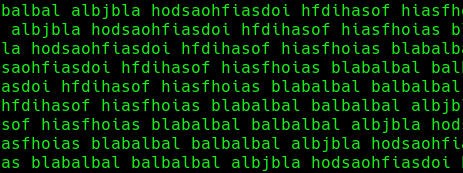
\includegraphics[width=\textwidth]{images/terminal.png}
        \caption{Original}
    \end{subfigure}
    \begin{subfigure}[]{0.49\textwidth}
        \centering
        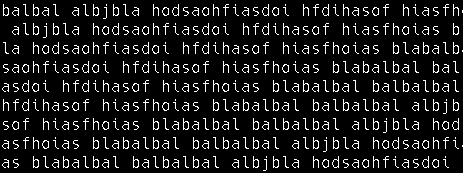
\includegraphics[width=\textwidth]{images/terminal_bin.png}
        \caption{Binarizado}
    \end{subfigure}
\end{figure}

\framebreak

\begin{figure}
    \centering
    \begin{subfigure}[]{0.49\textwidth}
        \centering
        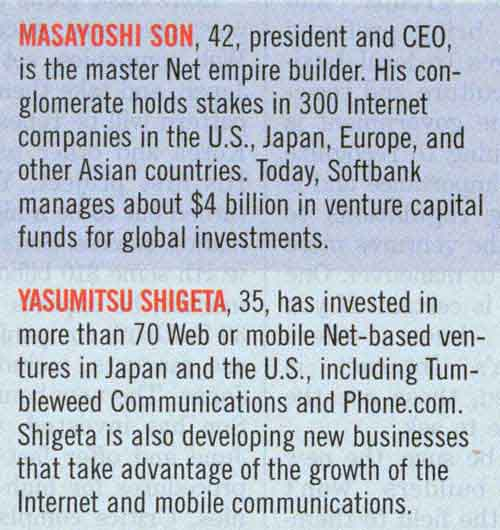
\includegraphics[width=\textwidth]{images/2.jpg}
        \caption{Original}
    \end{subfigure}
    \begin{subfigure}[]{0.49\textwidth}
        \centering
        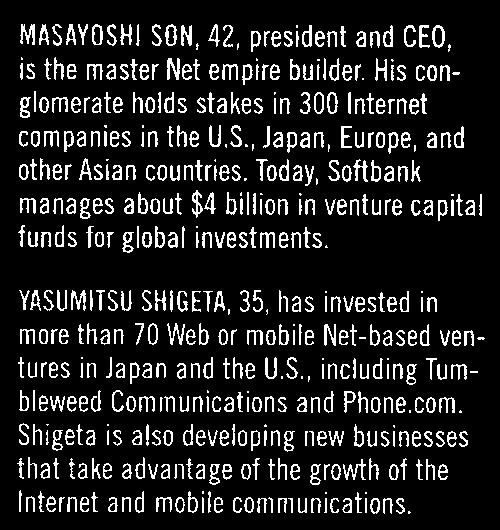
\includegraphics[width=\textwidth]{images/2_bin.jpg}
        \caption{Binarizado}
    \end{subfigure}
\end{figure}

\end{frame}

\begin{frame}{Segundo passo (opcional): dilatação horizontal}

\begin{figure}
    \centering
    \begin{subfigure}[]{0.49\textwidth}
        \centering
        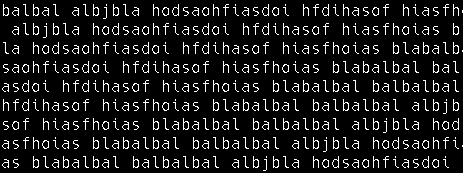
\includegraphics[width=\textwidth]{images/terminal_bin.png}
        \caption{Original binarizado}
    \end{subfigure}
    \begin{subfigure}[]{0.49\textwidth}
        \centering
        
\includegraphics[width=\textwidth]{images/terminal_dilated_5.png}
        \caption{n = 5}
    \end{subfigure}
    \begin{subfigure}[]{0.49\textwidth}
        \centering
        
\includegraphics[width=\textwidth]{images/terminal_dilated_10.png}
        \caption{n = 10}
    \end{subfigure}
    \begin{subfigure}[]{0.49\textwidth}
        \centering
        
\includegraphics[width=\textwidth]{images/terminal_dilated_20.png}
        \caption{n = 20}
    \end{subfigure}
\end{figure}

\end{frame}

\section{Algoritmo}

\begin{frame}{Algoritmo de segmentação de linhas (sem dilatação)}
    
\begin{enumerate}
    \item Demonstração no GIMP
    \item Percorre todas linhas horizontais de pixeis para verificar se tem texto ou não
    \item Limiar de contagem de pixeis para cada linha (de pixeis) definido como:
    $$se \ \frac{\sum{pixeis_{branco}}}{\sum{pixeis_{preto}}} >= limiar,$$
    Então linha de pixeis faz parte do texto e não do fundo.
\end{enumerate}

\end{frame}

\begin{frame}[allowframebreaks]{Resultados. Exemplo}

\begin{figure}
    \centering
    \begin{subfigure}[]{0.6\textwidth}
        \centering
        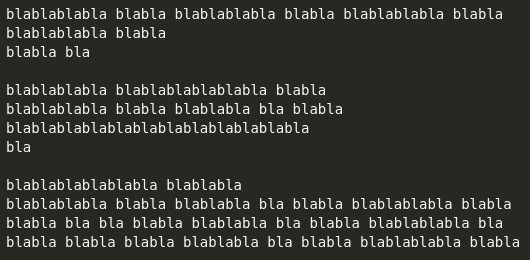
\includegraphics[width=\textwidth]{images/blabla.png}
        \caption{Original}
    \end{subfigure}
    \begin{subfigure}[]{0.6\textwidth}
        \centering
        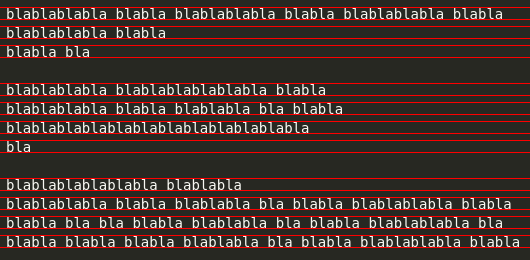
\includegraphics[width=\textwidth]{images/blabla_lines_001.png}
        \caption{Linhas segmentadas. Limiar = 0,1\%}
    \end{subfigure}
\end{figure}

\framebreak

\begin{figure}
    \centering
    \begin{subfigure}[]{0.49\textwidth}
        \centering
        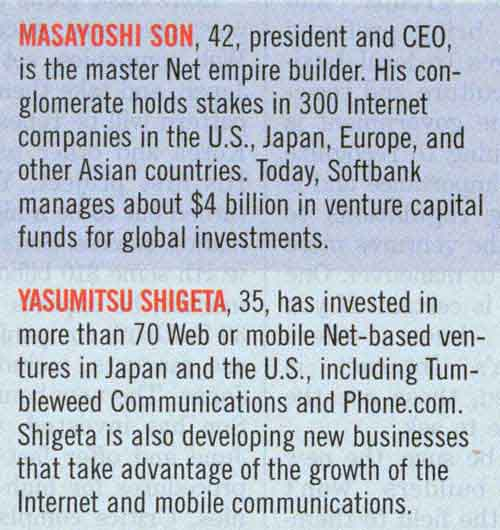
\includegraphics[width=\textwidth]{images/2.jpg}
        \caption{Original}
    \end{subfigure}
    \begin{subfigure}[]{0.49\textwidth}
        \centering
        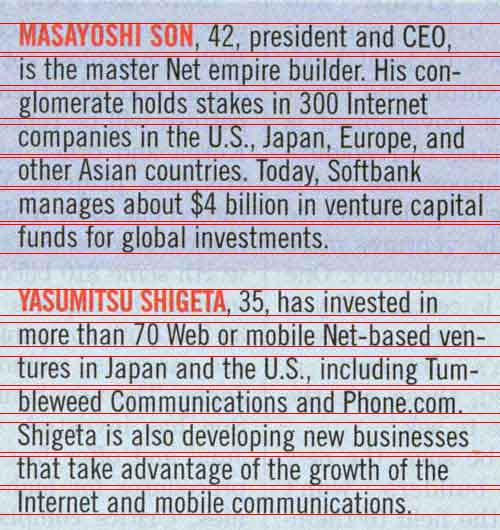
\includegraphics[width=\textwidth]{images/2_lines_001.jpg}
        \caption{Linhas segmentadas. Limiar = 0,1\%}
    \end{subfigure}
\end{figure}

\framebreak

\begin{figure}
    \centering
    \begin{subfigure}[]{0.49\textwidth}
        \centering
        
\includegraphics[width=\textwidth]{images/handwrite.png}
        \caption{Original}
    \end{subfigure}
    \begin{subfigure}[]{0.49\textwidth}
        \centering
        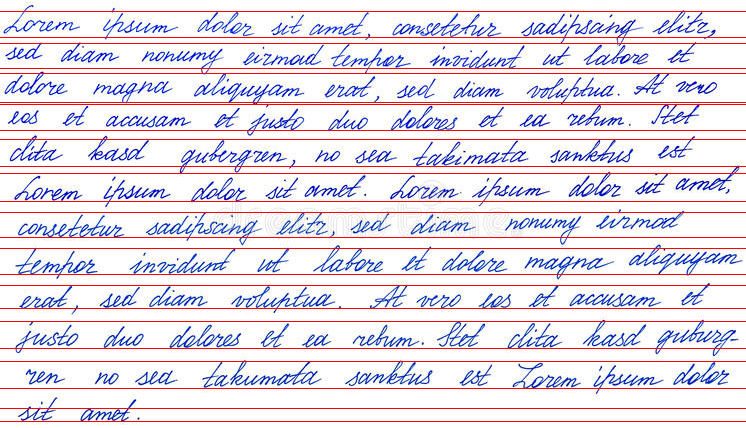
\includegraphics[width=\textwidth]{images/handwrite_lines_01.png}
        \caption{Linhas segmentadas. Limiar = 1\%}
    \end{subfigure}
\end{figure}

\framebreak

\begin{figure}
    \centering
    \begin{subfigure}[]{\textwidth}
        \centering
        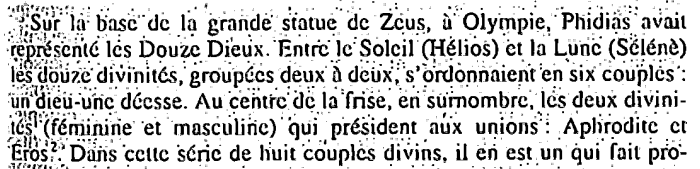
\includegraphics[width=\textwidth]{images/ruido.png}
        \caption{Original}
    \end{subfigure}
    \begin{subfigure}[]{\textwidth}
        \centering
        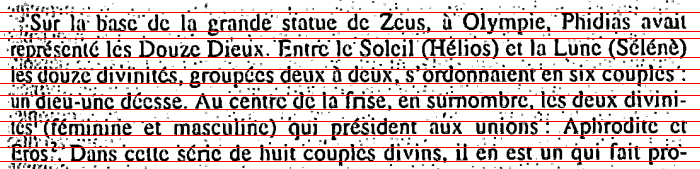
\includegraphics[width=\textwidth]{images/ruido_lines_10.png}
        \caption{Linhas segmentadas. Limiar = 10\%}
    \end{subfigure}
\end{figure}

\end{frame}

\begin{frame}{Segmentação de palavras (com dilatação)}
    
\begin{enumerate}
    \item Processo executado após segmentação das linhas (visto anteriormente)
    \item Exige dilatação
    \item Dentro de cada segmento de linha, verifica-se as colunas de pixeis para verificar se tem texto ou não
    \item Demonstração no GIMP
\end{enumerate}

\end{frame}

\begin{frame}[allowframebreaks]{Resultados. Exemplo}

\begin{figure}
    \centering
    \begin{subfigure}[]{0.49\textwidth}
        \centering
        
\includegraphics[width=\textwidth]{images/handwrite.png}
        \caption{Original}
    \end{subfigure}
    \begin{subfigure}[]{0.49\textwidth}
        \centering
        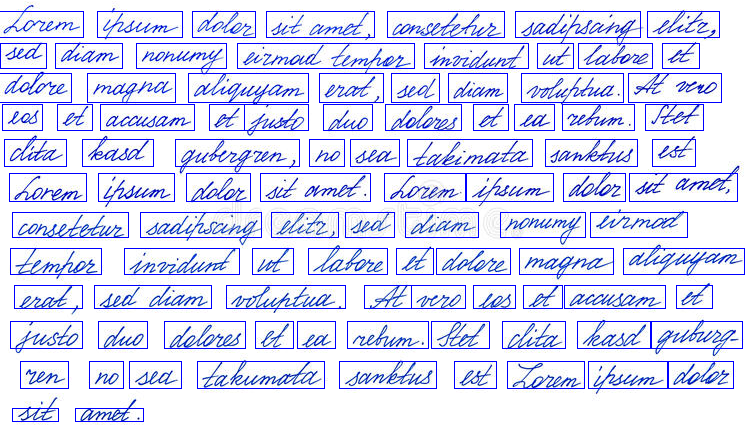
\includegraphics[width=\textwidth]{images/handwrite_words_10_01.png}
        \caption{Palavras segmentadas. N = 10 (dil.)}
    \end{subfigure}
\end{figure}

\framebreak

\begin{figure}
    \centering
    \begin{subfigure}[]{0.49\textwidth}
        \centering
        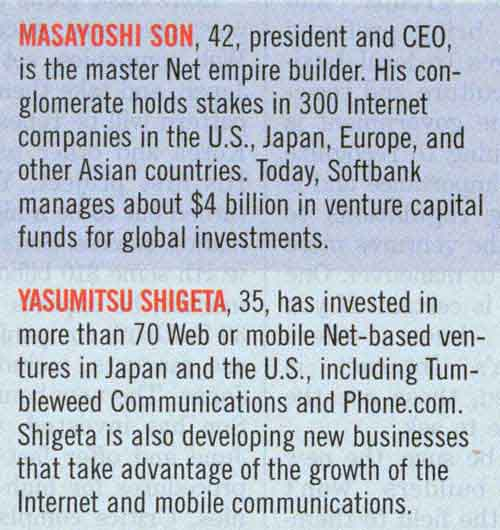
\includegraphics[width=\textwidth]{images/2.jpg}
        \caption{Original}
    \end{subfigure}
    \begin{subfigure}[]{0.49\textwidth}
        \centering
        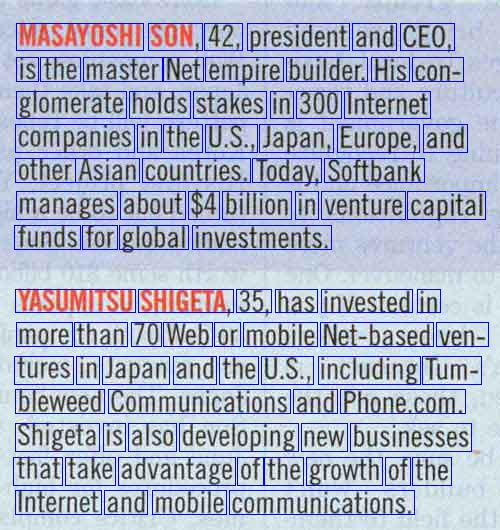
\includegraphics[width=\textwidth]{images/2_words_7_01.jpg}
        \caption{Palavras segmentadas. N = 7 (dil.)}
    \end{subfigure}
\end{figure}

\framebreak

\begin{figure}
    \centering
    \begin{subfigure}[]{0.6\textwidth}
        \centering
        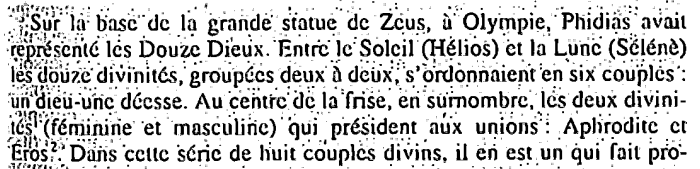
\includegraphics[width=\textwidth]{images/ruido.png}
        \caption{Original}
    \end{subfigure}
    \begin{subfigure}[]{0.6\textwidth}
        \centering
        
\includegraphics[width=\textwidth]{images/ruido_words_dilated.png}
        \caption{Palavras dilatadas, N = 6}
    \end{subfigure}
    \begin{subfigure}[]{0.6\textwidth}
        \centering
        
\includegraphics[width=\textwidth]{images/ruido_words_6_1.png}
        \caption{Palavras segmentadas (com erros)}
    \end{subfigure}
\end{figure}

\framebreak

\begin{figure}
    \centering
    \begin{subfigure}[]{\textwidth}
        \centering
        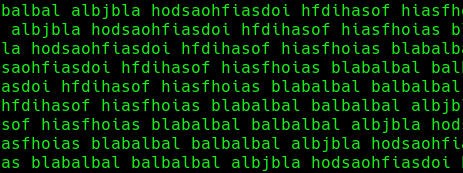
\includegraphics[width=0.7\textwidth]{images/terminal.png}
        \caption{Original}
    \end{subfigure}
    \begin{subfigure}[]{\textwidth}
        \centering
        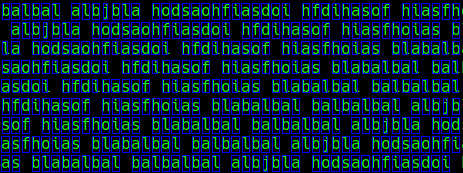
\includegraphics[width=0.7\textwidth]{images/terminal_words_1_001.png}
        \caption{Characteres segmentados, N = 1 (dil)}
    \end{subfigure}
\end{figure}

\end{frame}

\begin{frame}{Material}

\begin{itemize}
    \item \small{\url{https://github.com/RGNagel/line-segmentation-in-text-images}}
    \item \small{\url{https://github.com/RGNagel/apresentacao-SNCT-2020}}
\end{itemize}

\end{frame}

%------------------------------------------------

\begin{frame}
\Huge{\centerline{Fim}}
\end{frame}

%----------------------------------------------------------------------------------------

\end{document} 